\documentclass[tikz,border=2pt]{standalone}
\usepackage{amsmath}
\usetikzlibrary{arrows.meta}
\begin{document}
% Three-move centipede solved from the last node back: node 3 Stop (3>2) -> (3,1); node 2 Stop
% (2>1) -> (0,2); node 1 Stop (1>0) -> outcome (1,0). Chosen actions in green.
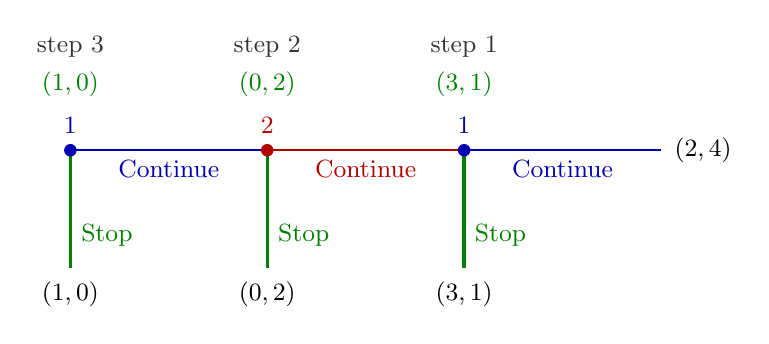
\begin{tikzpicture}[font=\small, >={Latex[length=2mm]},
    dec/.style={circle, fill, inner sep=1.6pt}]
  \def\d{2.5}
  % Continue edges (not chosen)
  \draw[thick, blue!70!black] (0,0) -- node[below, pos=0.5] {Continue} (\d,0);
  \draw[thick, red!70!black] (\d,0) -- node[below, pos=0.5] {Continue} (2*\d,0);
  \draw[thick, blue!70!black] (2*\d,0) -- node[below, pos=0.5] {Continue} (3*\d,0);
  % Stop edges (chosen)
  \foreach \i in {0,1,2}
    \draw[very thick, green!50!black] (\i*\d,0) -- node[right, pos=0.72] {Stop} (\i*\d,-1.5);
  % nodes and players
  \node[dec, blue!70!black, label={[blue!70!black]above:$1$}] at (0,0) {};
  \node[dec, red!70!black, label={[red!70!black]above:$2$}] at (\d,0) {};
  \node[dec, blue!70!black, label={[blue!70!black]above:$1$}] at (2*\d,0) {};
  % terminal payoffs
  \node[anchor=north] at (0,-1.55) {$(1,0)$};
  \node[anchor=north] at (\d,-1.55) {$(0,2)$};
  \node[anchor=north] at (2*\d,-1.55) {$(3,1)$};
  \node[anchor=west] at (3*\d+0.05,0) {$(2,4)$};
  % backward-induction values replacing each node
  \foreach \i/\v/\s in {0/{(1,0)}/3, 1/{(0,2)}/2, 2/{(3,1)}/1} {
    \node[green!50!black, anchor=south] at (\i*\d,0.55) {$\v$};
    \node[gray!40!black, anchor=south] at (\i*\d,1.05) {step $\s$};
  }
\end{tikzpicture}
\end{document}
